%Sección
\section{Bases de Datos}
\lhead[\thepage]{\thesection Bases de Datos}

\subsubsection{Definición}

Se puede definir una base de datos como un almacén de información actualizable de una aplicación, donde los aspectos físicos del almacenamiento y la representación de la información son transparentes al usuario. La información
almacenada en una base de datos es accesible a un nivel lógico sin necesidad de involucrar los
conceptos físicos de su complementación.\cite{6-josemy}

\subsection{Modelos de bases de datos} 

Las bases de datos pueden agruparse en modelos dependiendo de su estructura lógica y el modo como se almacenan, organizan y manipulan los datos. Se manejan principalmente dos tipos de modelos: las bases de
datos SQL y las bases de datos NoSQL.

\subsubsection{Bases de datos SQL}


Una base de datos relacional es aquella que presenta la información en tablas con filas y columnas. Una tabla es considerada como una relación, en el sentido de que es una colección de objetos de un mismo tipo (filas). Los datos en las tablas pueden estar relacionados de acuerdo a claves comunes o conceptos, y la habilidad de obtener datos relacionados de una tabla es la base del termino base de datos relacional.\cite{orcman}

La gestión de los datos, se  realiza a través de un lenguaje de consultas estructuradas (SQL), SQL permite realizar consultas interactivas con las cuales se extraerá o gestionará información de la base de datos \cite{25-carrejo}.

Algunas bases de datos relacionales conocidas son: MySQL, Oracle, PostgreSQL, MariaDB.

\subsubsection{Bases de datos NoSQL}

Con el objetivo de disminuir el acceso a la memoria secundaria del computador, hace unos años, los programadores comenzaron a utilizar distintas técnicas para almacenar los datos con mayor frecuencia de uso en la memoria RAM. Para lograr esto se basaron en un sistema donde todas las primitivas se escribían en forma clave/valor, además de las tradicionales consultas SQL en la
base de datos principal. Este enfoque les resulto de mayor comodidad a los desarrolladores, los cuales 
comenzaron a experimentar con bases de datos que utilizaban una interfaz de clave/valor para
el almacenamiento persistente, así como para la memoria caché, ya que la mayoría de sus consultas se expresaban de esa forma.\cite{dataglossary}

La interfaz de clave/valor representa la eliminación de una capa de abstracción al ser esta menos expresiva y de un nivel más bajo que un lenguaje como SQL. Estos sistemas aumenta la complejidad para el desarrollador, pero ofrecen mayor flexibilidad y control sobre el funcionamiento de la base de datos que se está manejando. También facilita a los desarrolladores de base de datos crear sistemas nuevos y experimentales para probar nuevas soluciones a requerimientos más complicados, como la escalabilidad, conjuntos de datos ampliamente distribuidos o aplicaciones de alto rendimiento.\cite{dataglossary}

En \cite{sprock}, Antonio Sprock profesor de la Universidad Central de Venezuela afirma :
\begin{quotation}
Muchos desarrolladores terminaron construyeron sus propias soluciones para almacenar datos,
y luego las publicaron como código abierto. Grandes industrias de internet, como Google,
Facebook, Twitter y Amazon han apostado a NoSQL, y defienden sus trabajos afirmando que:
no están utilizando una base de datos, sino “sistemas de almacenamiento distribuido para
gestionar datos estructurados”, se pueden ejecutar en clústers de servidores de computadoras
baratas, superan los cuellos de botella de rendimiento al manipular los grandes volúmenes de
datos, y evitan contar con mucho más de lo que puede cubrir sus necesidades. 

Por otro lado, NoSQL puede servir gran cantidad de carga de lecturas y escrituras. Implementaciones de NoSQL usadas en el mundo real incluyen los 6 TB de la base de datos del “ENSEMBLE” de la Comisión Europea usada en los modelos de comparación y calidad del aire, los nuevos 500 TB diarios de Facebook, entre sus 300 millones de nuevas fotos y los 2 billones de \textit{Likes} diarios, los 90 PB de eBay, los 51 TB de Amazon y los 2.5 PB de Walmart, entre otras.
\end{quotation}

Lo que indica que junto a Big Data, viene de la mano el auge de las bases de datos NoSQL como una forma de almacenamiento que aporta flexibilidad ante la cantidad masiva de datos que se generan hoy en día.


\subsubsection{Ventajas de bases de datos NoSQL} 
Esta forma de almacenar la información ofrece ciertas ventajas sobre los modelos relacionales. Entre las ventajas más significativas se pueden destacar:
\begin{itemize}
\item Se ejecutan en máquinas con pocos recursos.\cite{11-josemy}
\item Escalabilidad horizontal. \cite{11-josemy}
\item  Pueden manejar gran cantidad de datos, esto debido a que utilizan una estructura
distribuida.\cite{11-josemy}
\item  No genera cuellos de botella. \cite{11-josemy}
\end{itemize}
 

\subsubsection{Principales diferencias con las bases de datos SQL}
\begin{itemize}
\item  SQL no es su lenguaje principal de consultas: La mayoría de las base de datos NoSQL evitan utilizar el lenguaje SQL o lo utilizan como un lenguaje de soporte.\cite{11-josemy}
\item No utilizan estructuras fijas como tablas para el almacenamiento de los datos.\cite{11-josemy}
\item No suelen permitir operaciones JOIN: Al manejar volúmenes de datos masivos las operaciones JOIN presentan una carga muy elevada para el sistema. Esto se debe a que, cuando la operación no es la búsqueda de una clave, la sobrecarga puede llegar a ser muy costosa.\cite{11-josemy}
\item Arquitectura distribuida: La información puede estar compartida en varias máquinas mediante mecanismos de tablas \emph{hash} distribuidas. \cite{11-josemy}
\end{itemize}

\subsection{Los términos ACID y BASE}


En 1983, Andreas Reuter y Theo Härder publican el paper \emph{``Principles of Transaction-Oriented Database Recovery''} acuñando de forma oficial el termino ACID, dicho acronimo se define actualmente por los siguientes conceptos \cite{acidbase}:

\begin{itemize}
\item Atomicidad (\emph{Atomicity}): La tarea o todas las tareas en una transacción son realizadas o ninguna de ellas se realiza. Si un elemento de la transacción falla, toda la transacción lo hace.\cite{acidbase}
\item Consistencia (\emph{Consistency}): La transacción debe seguir todos los protocolos o reglas definidas por el sistema en todo momento. La transacción no viola estos protocolos y la base de datos debe permanecer en un estado consistente en el comienzo y final de una transacción, no habrá ninguna transacción a medio completar.\cite{acidbase}
\item Aislamiento (\emph{Isolation}): Ninguna transacción tendrá acceso a alguna otra que se encuentre en un estado intermedio o sin terminar. Por lo que cada transacción es independiente mientras se ejecuta.\cite{acidbase}
\item  Durabilidad (\emph{Durability}): Una vez la transacción esta completada, persistirá como completada y no puede ser deshacerse, sobrevivirá fallos en el sistema, perdida de energía y otro tipo de fallas.\cite{acidbase}
\end{itemize}
    
El concepto ACID es esencial en el ámbito de las bases de datos relacionales, sin el la fiabilidad es incierta.\cite{acidbase}


En el caso de los sistemas distribuidos que manejan grandes volumenes de datos, y deben lidiar con lo descrito en el teorema CAP, es necesario un enfoque distinto, por lo que surge BASE (\emph{Basically Available, Soft state, Eventual consistency})\cite{acidbase}:

\begin{itemize}
\item Basicamente Disponible (\emph{Basically Available}): El sistema garantiza la disponibilidad de los datos, habrá una respuesta a cualquier solicitud, pero esa respuesta puede tener fallas en obtener los datos solicitados, o, los mismos pueden contener inconsistencia o cambiado de estado.\cite{acidbase}

\item Estado suave (\emph{Soft state}: El estado del sistema puede cambiar con el tiempo, así que incluso durante tiempo sin operaciones de entrada, pueden estar sucediendo cambios debido a la consistencia eventual.\cite{acidbase} 

\item Consistencia Eventual (\emph{Eventual consistency}): El sistema sera eventualmente consistente, una vez deje de recibir operaciones de entrada.  Los datos se propagaran en todo el sistema tarde o temprano, pero el sistema continuara recibiendo operaciones de entrada y este no chequea la consistencia de cada transacción antes de moverse a la siguiente.\cite{acidbase}

\end{itemize}



\subsection{Tipos de bases de datos NoSQL}

Dependiendo de la forma en la que almacenen la información, se pueden encontrar varios tipos
distintos de bases de datos NoSQL. Los tipos más utilizados son:
\begin{itemize}

\begin{figure}[!htbp]
    \centering
    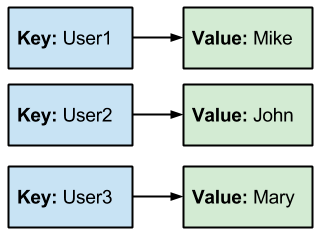
\includegraphics[width=0.5\textwidth]{Figuras/key_value.png}
    \caption{Arquitectura de base de dato Clave/Valor}
    \label{fig:arcclavevalor}
    \source{http://www.kdnuggets.com/wp-content/uploads/key-value.png}
\end{figure}

\item Bases de datos clave/valor: modelo mas utilizado entre las bases de datos NoSQL, tiene el funcionamiento mas sencillo. En este tipo de sistema, cada elemento se identifica por una clave única, lo que permite la recuperación de la información de forma rápida. Se caracterizan por ser muy eficientes tanto para las lecturas como para las escrituras.\cite{11-josemy}


\begin{figure}[!htbp]
    \centering
    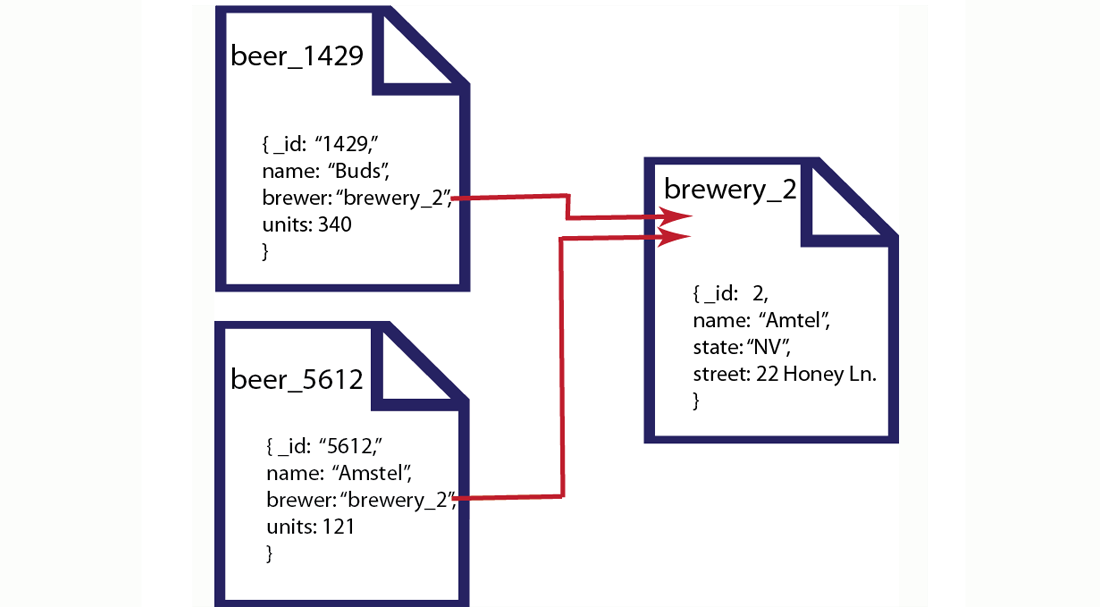
\includegraphics[width=0.8\textwidth]{Figuras/relating_docs.png}
    \caption{Arquitectura de base de dato orientada a documentos}
    \label{fig:arcdoc}
    \source{http://docs.couchbase.com/developer/dev-guide-3.0/images/relating\_docs.png}
\end{figure}

\item Bases de datos orientadas a documentos: la información es almacenada utilizando para ello una estructura simple como JSON o XML representando esta estructura al documento, cada registro es entonces asociado a un identificador único. Esta implementación permite realizar búsquedas por clave/valor y consultas avanzadas sobre el contenido del documento. Son las bases de datos NoSQL más versátiles. Se pueden utilizar en gran cantidad de proyectos, incluyendo muchos que tradicionalmente funcionarían sobre bases de datos relacionales.\cite{11-josemy}

\begin{figure}[!htbp]
    \centering
    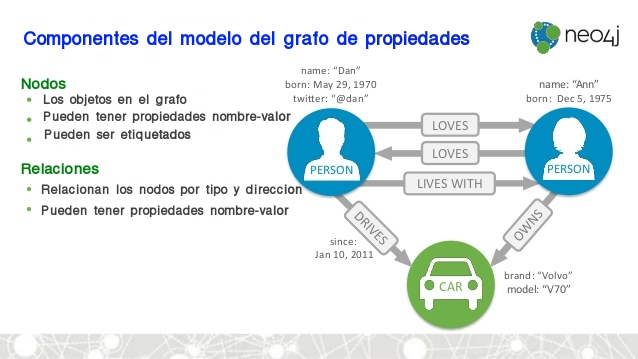
\includegraphics[width=1\textwidth]{Figuras/arcgraph.jpg}
    \caption{Arquitectura de base de dato en Grafo}
    \label{fig:arcgrpah}
    \source{http://image.slidesharecdn.com/rdbmstographsintro-150331090204-conversion-gate01/95/introduction-relational-to-graphs-13-638.jpg}
\end{figure}

\item Bases de datos en Grafo: En este tipo de bases de datos, la información se representa como nodos de un grafo y sus relaciones con las aristas del mismo, pudiendo explotarse la teoría de grafos para recorrerla \cite{11-josemy}.  A diferencia de otras bases de datos, las relaciones son la primera prioridad en las bases de datos en grafo \cite{neo4j}.

\begin{figure}[H]
    \centering
    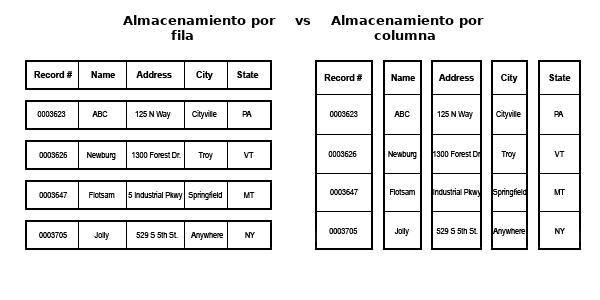
\includegraphics[width=0.7\textwidth]{Figuras/rowvcol.png}
    \caption{Base de datos tradicional vs columnar}
    \label{fig:rowvcol}
    \source{http://arxtecture.com/wp-content/uploads/2014/01/row-store-v-column-store.gif}
\end{figure}

\item Bases de datos columnares: Una base de datos columnar, también conocida como bases de datos orientadas a columnas, es una sistema manejador de base de datos que almacena los datos en columnas en vez de en filas, los datos que son almacenados aparecen en orden de guardado, lo que significa que el valor en la primera columna esta relacionado a el valor en la segunda y subsecuentes columnas si el mismo aparece en la misma fila \cite{technocolumnar}.Bajo este enfoque mejora la velocidad en recuperación de datos y operaciones que involucren los atributos de un objeto, mejorando mucho la lectura en la base de datos, sin embargo no es eficiente  al realizar escrituras a la base de datos, o cuando las operaciones involucran pocas columnas\cite{columnardb}. 


\end{itemize}

La versatilidad de las bases de datos NoSQL han originado la creacion de distintos manejadores con sus propios enfoques, la lista de bases de datos NoSQL sigue creciendo, a continuación se listan algunos de los mas utilizados:
\begin{itemize}
\item HBase : diseñado como un clon de código abierto del proyecto BigTable de Google, cuenta con una interfaz muy similar y comparten una alta compatibilidad. También utiliza un clon del sistema de archivos de Google (GFS) llamado Hadoop distributed file system (HDFS).\cite{dataglossary}

HBase está altamente integrado con el proyecto Apache Hadoop. La lectura y escritura a través de jobs MapReduce es fluida, sin embargo la latencia individual esta afectada por la carga implícita que tienen los sistemas distribuidos al lidiar con el trafico de red. El elemento fuerte de HBase se muestra cuando muchos clientes acceden de forma distribuida al sistema.\cite{dataglossary}

\item Apache Accumulo : es un almacén estructurado altamente escalable basado en BigTable de Google. Esta escrito en Java y opera sobre \emph{Hadoop Distributed File System (HDFS)}. Accumulo soporta un almacenamiento y recuperación eficiente de datos estructurados, incluidas búsquedas por rango, y provee soporte para usar las tablas de Accumulo como entras y salidas de unidades de trabajo MapReduce.\cite{manualacumulo}

Accumulo posee entre sus características balanceo de carga y particionado automático, compresión de datos y etiquetas de seguridad de grano fino.\cite{manualacumulo}

Accumulo almacena pares clave/valor ordenados. La ordenación de los datos por la clave
permite búsquedas rápidas de claves individuales o exploraciones de más de una serie de
claves. Puesto que los datos se recuperan por claves, éstas deben contener la información que
se utilizará para hacer la búsqueda. \cite{13}
El diseño original de BigTable tiene un paradigma de filas y columnas. Accumulo extiende las
columnas con una etiqueta adicional, conocida como "visibilidad", la cual proporciona el control
de acceso de grano fino.\cite{13}


\item Cassandra: Es un sistema de clave/valor distribuido, con valores muy estructurados que se realizan en una
jerarquía similar a los niveles de base de datos clásicas. Por defecto, los datos son fragmentados y equilibrados
automáticamente usando un \emph{hashing} consistente en rangos de clave, aunque permite configurar otros esquemas. \cite{dataglossary}
 Las estructuras de datos están optimizadas para un rendimiento de escritura consistente, al costo de lecturas lentas ocasionales. Una de sus características mas útil es la habilidad de especificar cuantos nodos deben aceptar antes de completas una operación de lectura o escritura. Configurar el nivel de consistencia permite ajustar las concesiones entre la disponibilidad y tolerancia a partición, para priorizas rapidez sobre consistencia o viceversa.\cite{dataglossary}

\item MongoDB: Es una base de datos orientada a documentos, con registros que son similares a objetos JSON con la habilidad de almacenar y consultar sobre atributos anidados \cite{dataglossary}.MongoDB ha sido creada para brindar escalabilidad, rendimiento y gran disponibilidad,
escalando de una implantación de servidor único a grandes arquitecturas complejas de centros multidatos. MongoDB brinda un elevado rendimiento, tanto para lectura como para escritura, potenciando la computación en memoria. La replicación nativa de MongoDB y la
tolerancia a fallos automática ofrece fiabilidad a nivel empresarial y flexibilidad operativa \cite{mongo}.

\item Redis : Dos características sobresalen en Redis: mantiene la base de datos entera en la RAM, y sus valores pueden ser estructuras de datos complejas. Aunque la estructura completa se mantiene en la RAM, es periódicamente respaldada en disco, por lo que se puede usar como una base de datos persistente. Este enfoque ofrece un rendimiento rápido y predecible, pero las velocidades caen si los datos se expanden mas allá de las capacidades de la RAM.\cite{dataglossary}

 \cite{11-josemy}
\end{itemize}

